% Options for packages loaded elsewhere
\PassOptionsToPackage{unicode}{hyperref}
\PassOptionsToPackage{hyphens}{url}
\PassOptionsToPackage{dvipsnames,svgnames,x11names}{xcolor}
%
\documentclass[
  letterpaper,
  DIV=11,
  numbers=noendperiod]{scrartcl}

\usepackage{amsmath,amssymb}
\usepackage{iftex}
\ifPDFTeX
  \usepackage[T1]{fontenc}
  \usepackage[utf8]{inputenc}
  \usepackage{textcomp} % provide euro and other symbols
\else % if luatex or xetex
  \usepackage{unicode-math}
  \defaultfontfeatures{Scale=MatchLowercase}
  \defaultfontfeatures[\rmfamily]{Ligatures=TeX,Scale=1}
\fi
\usepackage{lmodern}
\ifPDFTeX\else  
    % xetex/luatex font selection
\fi
% Use upquote if available, for straight quotes in verbatim environments
\IfFileExists{upquote.sty}{\usepackage{upquote}}{}
\IfFileExists{microtype.sty}{% use microtype if available
  \usepackage[]{microtype}
  \UseMicrotypeSet[protrusion]{basicmath} % disable protrusion for tt fonts
}{}
\makeatletter
\@ifundefined{KOMAClassName}{% if non-KOMA class
  \IfFileExists{parskip.sty}{%
    \usepackage{parskip}
  }{% else
    \setlength{\parindent}{0pt}
    \setlength{\parskip}{6pt plus 2pt minus 1pt}}
}{% if KOMA class
  \KOMAoptions{parskip=half}}
\makeatother
\usepackage{xcolor}
\setlength{\emergencystretch}{3em} % prevent overfull lines
\setcounter{secnumdepth}{-\maxdimen} % remove section numbering
% Make \paragraph and \subparagraph free-standing
\makeatletter
\ifx\paragraph\undefined\else
  \let\oldparagraph\paragraph
  \renewcommand{\paragraph}{
    \@ifstar
      \xxxParagraphStar
      \xxxParagraphNoStar
  }
  \newcommand{\xxxParagraphStar}[1]{\oldparagraph*{#1}\mbox{}}
  \newcommand{\xxxParagraphNoStar}[1]{\oldparagraph{#1}\mbox{}}
\fi
\ifx\subparagraph\undefined\else
  \let\oldsubparagraph\subparagraph
  \renewcommand{\subparagraph}{
    \@ifstar
      \xxxSubParagraphStar
      \xxxSubParagraphNoStar
  }
  \newcommand{\xxxSubParagraphStar}[1]{\oldsubparagraph*{#1}\mbox{}}
  \newcommand{\xxxSubParagraphNoStar}[1]{\oldsubparagraph{#1}\mbox{}}
\fi
\makeatother


\providecommand{\tightlist}{%
  \setlength{\itemsep}{0pt}\setlength{\parskip}{0pt}}\usepackage{longtable,booktabs,array}
\usepackage{calc} % for calculating minipage widths
% Correct order of tables after \paragraph or \subparagraph
\usepackage{etoolbox}
\makeatletter
\patchcmd\longtable{\par}{\if@noskipsec\mbox{}\fi\par}{}{}
\makeatother
% Allow footnotes in longtable head/foot
\IfFileExists{footnotehyper.sty}{\usepackage{footnotehyper}}{\usepackage{footnote}}
\makesavenoteenv{longtable}
\usepackage{graphicx}
\makeatletter
\newsavebox\pandoc@box
\newcommand*\pandocbounded[1]{% scales image to fit in text height/width
  \sbox\pandoc@box{#1}%
  \Gscale@div\@tempa{\textheight}{\dimexpr\ht\pandoc@box+\dp\pandoc@box\relax}%
  \Gscale@div\@tempb{\linewidth}{\wd\pandoc@box}%
  \ifdim\@tempb\p@<\@tempa\p@\let\@tempa\@tempb\fi% select the smaller of both
  \ifdim\@tempa\p@<\p@\scalebox{\@tempa}{\usebox\pandoc@box}%
  \else\usebox{\pandoc@box}%
  \fi%
}
% Set default figure placement to htbp
\def\fps@figure{htbp}
\makeatother

\KOMAoption{captions}{tableheading}
\makeatletter
\@ifpackageloaded{caption}{}{\usepackage{caption}}
\AtBeginDocument{%
\ifdefined\contentsname
  \renewcommand*\contentsname{Table of contents}
\else
  \newcommand\contentsname{Table of contents}
\fi
\ifdefined\listfigurename
  \renewcommand*\listfigurename{List of Figures}
\else
  \newcommand\listfigurename{List of Figures}
\fi
\ifdefined\listtablename
  \renewcommand*\listtablename{List of Tables}
\else
  \newcommand\listtablename{List of Tables}
\fi
\ifdefined\figurename
  \renewcommand*\figurename{Figure}
\else
  \newcommand\figurename{Figure}
\fi
\ifdefined\tablename
  \renewcommand*\tablename{Table}
\else
  \newcommand\tablename{Table}
\fi
}
\@ifpackageloaded{float}{}{\usepackage{float}}
\floatstyle{ruled}
\@ifundefined{c@chapter}{\newfloat{codelisting}{h}{lop}}{\newfloat{codelisting}{h}{lop}[chapter]}
\floatname{codelisting}{Listing}
\newcommand*\listoflistings{\listof{codelisting}{List of Listings}}
\makeatother
\makeatletter
\makeatother
\makeatletter
\@ifpackageloaded{caption}{}{\usepackage{caption}}
\@ifpackageloaded{subcaption}{}{\usepackage{subcaption}}
\makeatother

\usepackage{bookmark}

\IfFileExists{xurl.sty}{\usepackage{xurl}}{} % add URL line breaks if available
\urlstyle{same} % disable monospaced font for URLs
\hypersetup{
  pdftitle={Financial Markets: Part III},
  pdfauthor={Prof.~Ji-Woong Chung},
  colorlinks=true,
  linkcolor={blue},
  filecolor={Maroon},
  citecolor={Blue},
  urlcolor={Blue},
  pdfcreator={LaTeX via pandoc}}


\title{Financial Markets: Part III}
\usepackage{etoolbox}
\makeatletter
\providecommand{\subtitle}[1]{% add subtitle to \maketitle
  \apptocmd{\@title}{\par {\large #1 \par}}{}{}
}
\makeatother
\subtitle{BUSS254 Investments}
\author{Prof.~Ji-Woong Chung}
\date{}

\begin{document}
\maketitle


\subsection{Lecture Outline}\label{lecture-outline}

\begin{itemize}
\tightlist
\item
  Money markets: Call, Repo, CD, CP, etc.
\item
  Capital markets: Bond, Equity
\item
  Derivatives markets: Futures, options etc.
\item
  Trading mechanisms
\item
  Investment Companies
\item
  Reading: BKM Ch. 3 and 4
\end{itemize}

\begin{center}\rule{0.5\linewidth}{0.5pt}\end{center}

\subsection{Trading Mechanics}\label{trading-mechanics}

\subsubsection{Why Trade?}\label{why-trade}

\begin{itemize}
\tightlist
\item
  \textbf{Information-driven trading}: Traders act on private or public
  information.
\item
  \textbf{Non-information-driven trading}:

  \begin{itemize}
  \tightlist
  \item
    \textbf{Hedging}: Reducing risk exposure.
  \item
    \textbf{Liquidity needs}: Buying or selling for cash flow reasons.
  \end{itemize}
\item
  \textbf{Noise trading}: Trading without fundamental justification,
  often irrational or random.
\end{itemize}

\subsubsection{Types of Orders}\label{types-of-orders}

\begin{itemize}
\tightlist
\item
  \textbf{Market order}: Executes immediately at the best available
  price.

  \begin{itemize}
  \tightlist
  \item
    Quick execution vs.~Price uncertainty.
  \end{itemize}
\item
  \textbf{Limit order}: Specifies price and waits for execution at that
  price or better.

  \begin{itemize}
  \tightlist
  \item
    Price control vs.~Execution uncertainty.
  \end{itemize}
\item
  \textbf{Stop order}: Becomes a market order once the stop price is
  triggered.

  \begin{itemize}
  \tightlist
  \item
    \textbf{Stop-loss}: Sells when the price falls below a set level.
  \item
    \textbf{Stop-buy}: Buys when the price rises above a set level.
  \end{itemize}
\item
  \textbf{Short selling}: Selling borrowed shares to profit from a price
  decline.
\item
  \textbf{Margin trading}: Borrowing funds to amplify trading positions,
  increasing both potential gains and risks.
\end{itemize}

\begin{center}\rule{0.5\linewidth}{0.5pt}\end{center}

\subsection{Margin Trading}\label{margin-trading}

\begin{itemize}
\tightlist
\item
  \textbf{Margin Purchase} = Borrowing + Investor's Equity
\item
  \textbf{Initial Margin}: Minimum equity required to open a position.
\item
  \textbf{Maintenance Margin}: Minimum equity required to keep the
  position open.
\item
  \textbf{Margin Call}: If the value of securities falls too much, the
  investor must:

  \begin{itemize}
  \tightlist
  \item
    Deposit more equity (\(\ge\) initial margin), or
  \item
    Liquidate the position.
  \end{itemize}
\end{itemize}

\begin{center}\rule{0.5\linewidth}{0.5pt}\end{center}

\subsection{Margin Trading: Example}\label{margin-trading-example}

\begin{itemize}
\tightlist
\item
  \textbf{Stock Price}: \$100 per share
\item
  \textbf{Shares Purchased}: 100
\item
  \textbf{Initial Margin}: 60\%
\item
  \textbf{Maintenance Margin}: 30\%
\end{itemize}

Initial Position:

\begin{longtable}[]{@{}llll@{}}
\toprule\noalign{}
Asset & Value & Liability & Equity \\
\midrule\noalign{}
\endhead
\bottomrule\noalign{}
\endlastfoot
Stock & \$10,000 & Borrowed & \$4,000 \\
& & Investor Equity & \$6,000 \\
\end{longtable}

If Stock Price Falls to \$70:

\begin{longtable}[]{@{}llll@{}}
\toprule\noalign{}
Asset & Value & Liability & Equity \\
\midrule\noalign{}
\endhead
\bottomrule\noalign{}
\endlastfoot
Stock & \$7,000 & Borrowed & \$4,000 \\
& & Investor Equity & \$3,000 \\
\end{longtable}

\begin{itemize}
\tightlist
\item
  \textbf{Margin\%} = Equity / Market Value =
  \(\frac{\$3,000}{\$7,000} = 43\%\)

  \begin{itemize}
  \tightlist
  \item
    Since 43\% \textgreater{} 30\% (maintenance margin), no margin call.
  \end{itemize}
\end{itemize}

\begin{center}\rule{0.5\linewidth}{0.5pt}\end{center}

\subsection{Margin Trading: Maintenance
Margin}\label{margin-trading-maintenance-margin}

How far can the stock price fall before a margin call?

\begin{itemize}
\item
  \textbf{Maintenance Margin} = 30\%
\item
  \textbf{Formula for Equity}:
  \(\text{Equity} = \text{Market Value} - \text{Borrowed Amount} = 100P - 4,000\)
\item
  \textbf{Margin\% Formula}: \(\frac{100P - 4,000}{100P} = 0.30\)
\item
  \textbf{Solving for Price}:
\end{itemize}

\[100P - 4,000 = 30P\] \[70P = 4,000\] \[P = 57.14\]

\begin{center}\rule{0.5\linewidth}{0.5pt}\end{center}

\subsection{Short Sales}\label{short-sales}

\begin{itemize}
\item
  Selling securities that you do not own to profit from a decline in the
  price of the securities

  \begin{enumerate}
  \def\labelenumi{\arabic{enumi}.}
  \tightlist
  \item
    \textbf{Borrow securities} through a dealer or broker.
  \item
    \textbf{Sell them} and deposit the proceeds along with the margin in
    an account.

    \begin{itemize}
    \tightlist
    \item
      You \textbf{cannot withdraw} the proceeds until you ``cover'' the
      position.
    \end{itemize}
  \item
    \textbf{Closing out the position}: Buy back the securities and
    return them to the lender.
  \end{enumerate}
\item
  Naked short-selling:

  \begin{itemize}
  \tightlist
  \item
    Selling shares \textbf{without borrowing them first}, assuming they
    can be acquired later.
  \item
    \textbf{Illegal} due to the risk of delivery failure.
  \end{itemize}
\end{itemize}

\begin{center}\rule{0.5\linewidth}{0.5pt}\end{center}

\subsection{Short Sales: Example}\label{short-sales-example}

\begin{itemize}
\tightlist
\item
  \textbf{Stock X}: 1000 shares
\item
  \textbf{Initial Price}: \$100 per share
\item
  \textbf{Initial Margin}: 50\%
\item
  \textbf{Maintenance Margin}: 30\%
\end{itemize}

Position Setup:

\begin{longtable}[]{@{}ll@{}}
\toprule\noalign{}
Item & Value \\
\midrule\noalign{}
\endhead
\bottomrule\noalign{}
\endlastfoot
\textbf{Sale Proceeds} & \$100,000 \\
\textbf{Initial Margin} & \$50,000 \\
\textbf{Stock Owed} & 1000 shares \\
\end{longtable}

Balance Sheet:

\begin{longtable}[]{@{}ll@{}}
\toprule\noalign{}
\textbf{Assets} & \textbf{Liabilities} \\
\midrule\noalign{}
\endhead
\bottomrule\noalign{}
\endlastfoot
\$100,000 (sale proceeds) & \$100,000 (shares owed) \\
\$50,000 (initial margin) & \\
& \textbf{Equity} \\
& \$50,000 \\
\end{longtable}

\begin{center}\rule{0.5\linewidth}{0.5pt}\end{center}

\subsection{Short Sales: Example
(cont'd)}\label{short-sales-example-contd}

\begin{itemize}
\tightlist
\item
  If Price Falls to \textbf{\$70 per share}:
\end{itemize}

\begin{longtable}[]{@{}ll@{}}
\toprule\noalign{}
\textbf{Assets} & \textbf{Liabilities} \\
\midrule\noalign{}
\endhead
\bottomrule\noalign{}
\endlastfoot
\$100,000 (sales proceeds) & \$70,000 (shares) \\
\$50,000 (initial margin) & \\
& \textbf{Equity} \\
& \$80,000 \\
\end{longtable}

\begin{itemize}
\tightlist
\item
  Profit Calculation:
\end{itemize}

\[\text{Profit} = \text{Ending Equity} - \text{Beginning Equity}\]

\[= \$80,000 - \$50,000 = \$30,000\]

\[= (\text{Initial Price} - \text{New Price}) \times \text{Shares Sold Short}\]

\[= (100 - 70) \times 1000 = \$30,000\]

\begin{center}\rule{0.5\linewidth}{0.5pt}\end{center}

\subsection{Short Sales: Example
(cont'd)}\label{short-sales-example-contd-1}

\begin{itemize}
\tightlist
\item
  Maximum Stock Price Before Margin Call:
\item
  \textbf{Formula}:
\end{itemize}

\[\text{Margin%} = \frac{\text{Assets} - \text{Liabilities}}{\text{Market Value}}
\]

\[= \frac{(\$150,000 - 1000P)}{1000P} = 0.30\]

\begin{itemize}
\tightlist
\item
  \textbf{Solving for P}:
\end{itemize}

\[150,000 - 1000P = 0.30 \times 1000P\]

\[150,000 = 1300P\]

\[P = 115.38\]

\begin{itemize}
\tightlist
\item
  \(150,000\): Initial margin plus sale proceeds
\end{itemize}

\begin{center}\rule{0.5\linewidth}{0.5pt}\end{center}

\subsection{Trading Mechanisms}\label{trading-mechanisms}

\textbf{Auction Market}

\begin{itemize}
\tightlist
\item
  \textbf{Centralized}: Investors interact directly.
\item
  Orders are consolidated in a \textbf{limit order book (LOB)}:

  \begin{itemize}
  \tightlist
  \item
    \textbf{Bid} (buy) and \textbf{ask} (sell) orders.
  \end{itemize}
\item
  \textbf{Order-driven market}: Limit orders determine prices.
\item
  \textbf{Examples}: NYSE, Paris, Milan, Tokyo, Korea.
\end{itemize}

\textbf{Dearler Market}

\begin{itemize}
\tightlist
\item
  \textbf{Decentralized}: Trades occur via dealers.
\item
  Dealers quote \textbf{bid-ask prices}, taking on inventory risk.
\item
  \textbf{Quote-driven market}: Dealers set prices.
\item
  \textbf{Examples}: Nasdaq, bond markets, forex markets.
\end{itemize}

\begin{center}\rule{0.5\linewidth}{0.5pt}\end{center}

\subsection{Auction Market}\label{auction-market}

\pandocbounded{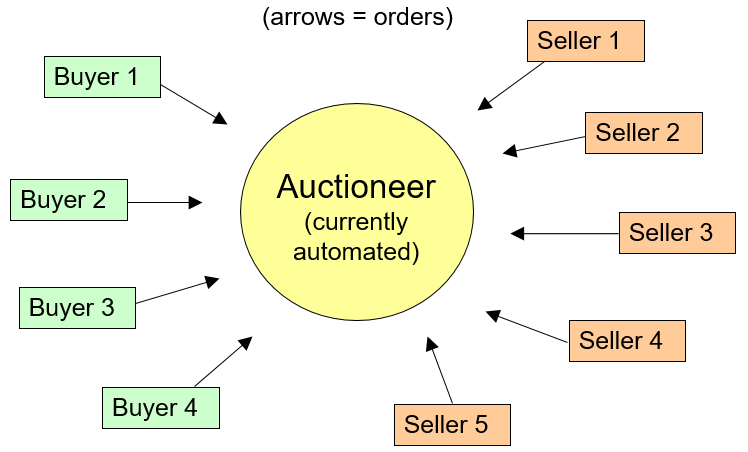
\includegraphics[keepaspectratio]{img/market_AuctionMarket.png}}

\begin{itemize}
\tightlist
\item
  \textbf{Call (Batch) Auction}: Orders are grouped and executed at
  specific times.

  \begin{itemize}
  \tightlist
  \item
    Typically at market \textbf{open} and \textbf{close}.
  \item
    Helps \textbf{reduce price distortions} from temporary order
    imbalances.
  \end{itemize}
\item
  \textbf{Continuous Auction}: Trading happens \textbf{continuously}
  throughout the day.
\end{itemize}

\begin{center}\rule{0.5\linewidth}{0.5pt}\end{center}

\subsection{Call Auction}\label{call-auction}

\pandocbounded{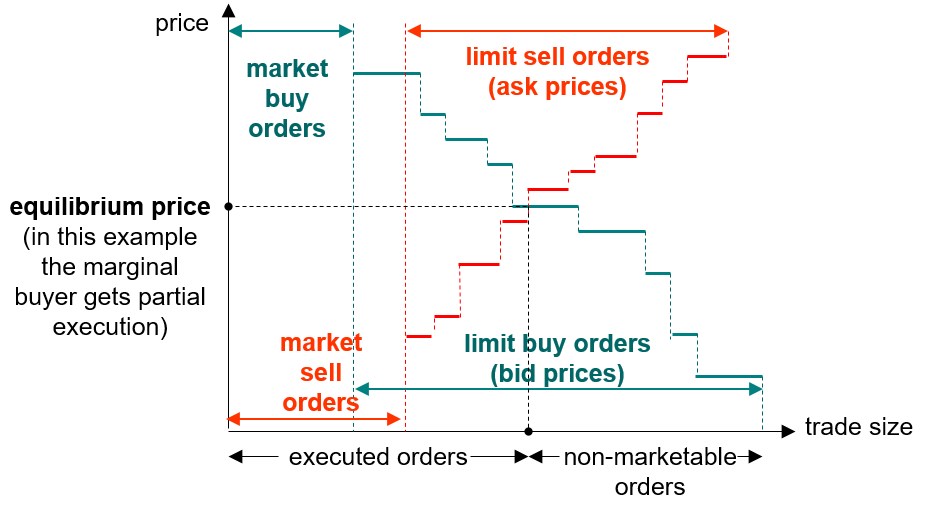
\includegraphics[keepaspectratio]{img//market_CallAuction.png}}

Buy orders sorted by decreasing price (demand), and sell orders by
increasing price (supply).

\begin{center}\rule{0.5\linewidth}{0.5pt}\end{center}

\subsection{Call Auction (cont'd)}\label{call-auction-contd}

\pandocbounded{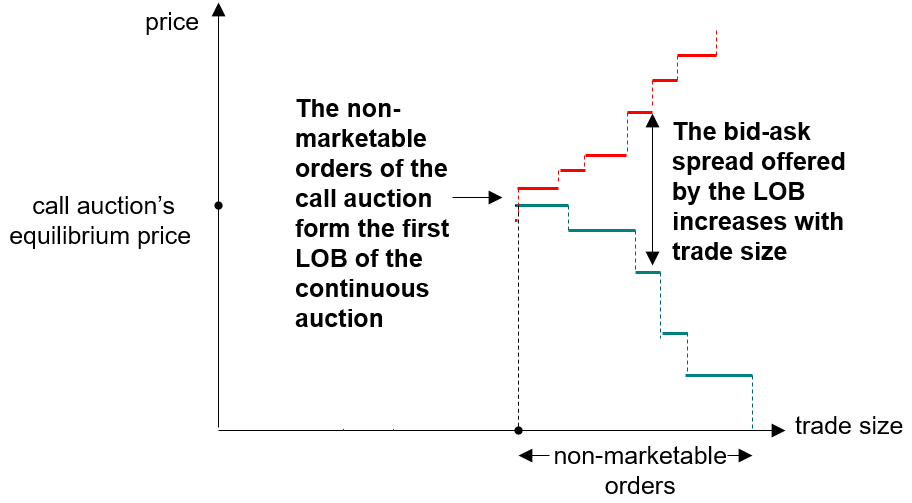
\includegraphics[keepaspectratio]{img//market_AfterCallAuction.png}}

Price set so that supply = demand. All executable orders are filled at
that price

\begin{center}\rule{0.5\linewidth}{0.5pt}\end{center}

\subsection{Continuous Auction: Limit Order
Book}\label{continuous-auction-limit-order-book}

\begin{itemize}
\tightlist
\item
  \textbf{Non-marketable orders} (those not executed in the call
  auction) enter the \textbf{Limit Order Book (LOB)}.
\item
  Incoming orders \textbf{execute against the LOB} based on:

  \begin{itemize}
  \tightlist
  \item
    \textbf{Price priority}: Best prices executed first.
  \item
    \textbf{Time priority}: Older orders executed before newer ones at
    the same price.
  \end{itemize}
\end{itemize}

\begin{longtable}[]{@{}llllll@{}}
\toprule\noalign{}
Bid & & & Ask & & \\
\midrule\noalign{}
\endhead
\bottomrule\noalign{}
\endlastfoot
Price & Size & Time & Price & Size & Time \\
74.42 & 300 & 11:49:39 & 74.48 & 300 & 11:49:35 \\
74.41 & 100 & 11:46:55 & 74.48 & 500 & 11:49:50 \\
74.36 & 400 & 11:48:30 & 75.74 & 100 & 08:25:17 \\
74.36 & 400 & 11:48:32 & 76.00 & 150 & 08:02:02 \\
\end{longtable}

\begin{itemize}
\tightlist
\item
  Market sell order of 200 (or limit sell with price \(<\) 74.42)
\item
  Market buy order of 900 (or limit buy with price \(>\) 75.74)
\item
  Because of the two orders, the bid-ask spread widens from
  \(74.48 - 74.42 = 0.06\) to \(76.00 - 74.42 = 1.58\).

  \begin{itemize}
  \tightlist
  \item
    \textbf{The two orders have ``consumed'' liquidity.}
  \end{itemize}
\item
  Market liquidity: the ability to trade securities quickly at a price
  close to its consensus value
\end{itemize}

\begin{center}\rule{0.5\linewidth}{0.5pt}\end{center}

\subsection{Dark Pools}\label{dark-pools}

\begin{itemize}
\item
  Electronic trading platforms accessible only to institutional
  investors.

  \begin{itemize}
  \tightlist
  \item
    Operated by stock exchanges (e.g., Turquoise by the LSE, Smartpool
    by Euronext, or Xetra by the Deutsche Börse), brokers (e.g.,
    BlockCross by ICAP or Blockmatch by Instinet) or banks (e.g., SigmaX
    by Goldman Sachs or SG CIB AlphaY by Société Générale).
  \item
    Operate in parallel with continuous limit order markets and offer
    investors an alternative way to execute their orders.
  \end{itemize}
\item
  Generally, dark pools do not contribute to price discovery

  \begin{itemize}
  \tightlist
  \item
    Reference prices drawn from other markets
  \end{itemize}
\item
  ``Dark'': orders are not displayed to the rest of market participants.

  \begin{itemize}
  \tightlist
  \item
    Reduces the risk of information leakage
  \end{itemize}
\end{itemize}

\begin{center}\rule{0.5\linewidth}{0.5pt}\end{center}

\subsection{Dealer Market}\label{dealer-market}

In dealer markets, investors do not trade directly with each other, but
must contact a dealer, find out his price, and trade at this price, or
else try another dealer.

\pandocbounded{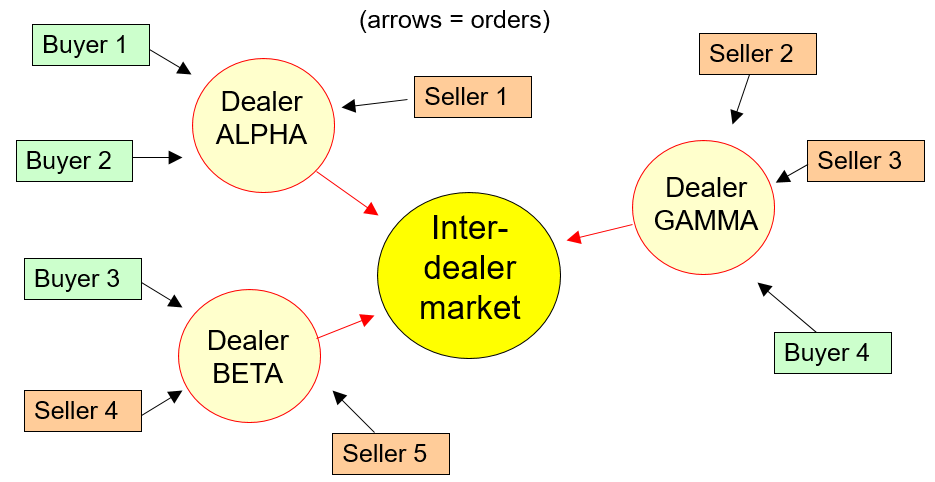
\includegraphics[keepaspectratio]{img//market_DealerMarket.png}}

\begin{center}\rule{0.5\linewidth}{0.5pt}\end{center}

\subsection{Dealer Market: Example}\label{dealer-market-example}

\begin{longtable}[]{@{}
  >{\raggedright\arraybackslash}p{(\linewidth - 8\tabcolsep) * \real{0.2424}}
  >{\raggedright\arraybackslash}p{(\linewidth - 8\tabcolsep) * \real{0.1970}}
  >{\raggedright\arraybackslash}p{(\linewidth - 8\tabcolsep) * \real{0.2273}}
  >{\raggedright\arraybackslash}p{(\linewidth - 8\tabcolsep) * \real{0.2121}}
  >{\raggedright\arraybackslash}p{(\linewidth - 8\tabcolsep) * \real{0.1212}}@{}}
\toprule\noalign{}
\begin{minipage}[b]{\linewidth}\raggedright
\textbf{Market Maker}
\end{minipage} & \begin{minipage}[b]{\linewidth}\raggedright
\textbf{Bid Price}
\end{minipage} & \begin{minipage}[b]{\linewidth}\raggedright
\textbf{Offer Price}
\end{minipage} & \begin{minipage}[b]{\linewidth}\raggedright
\textbf{Quote Size}
\end{minipage} & \begin{minipage}[b]{\linewidth}\raggedright
\textbf{Time}
\end{minipage} \\
\midrule\noalign{}
\endhead
\bottomrule\noalign{}
\endlastfoot
ALPHA & 326 & 330 & 75 × 75 & 8:53 \\
BETA & 324 & 330 & 75 × 75 & 9:14 \\
GAMMA & 325 & 329 & 75 × 75 & 9:16 \\
DELTA & 323 & 332 & 75 × 75 & 8:53 \\
EPSILON & 325 & 329 & 25 × 25 & 9:36 \\
ZETA & 326 & 330 & 75 × 75 & 11:30 \\
ETA & 325 & 330 & 75 × 75 & 9:45 \\
THETA & 325 & 330 & 75 × 75 & 9:23 \\
IOTA & 324 & 329 & 75 × 75 & 10:27 \\
KAPPA & 323 & 330 & 75 × 75 & 9:45 \\
LAMBDA & 325 & 330 & 75 × 75 & 8:53 \\
\end{longtable}

\begin{itemize}
\tightlist
\item
  \textbf{Seller 4} wants to sell \textbf{60 shares}.
\item
  Contacts \textbf{Dealer Beta}, who quotes \textbf{Bid = \$324, Ask =
  \$330}.
\item
  Seller 4 \textbf{can sell at \$324} or try another dealer.
\item
  \textbf{Inventory Risk}: Dealers face the risk of price drops after
  acquiring shares.
\end{itemize}

\begin{center}\rule{0.5\linewidth}{0.5pt}\end{center}

\subsection{Dealer Market (cont'd)}\label{dealer-market-contd}

\subsubsection{\texorpdfstring{\textbf{Key Differences from Limit Order
Markets}}{Key Differences from Limit Order Markets}}\label{key-differences-from-limit-order-markets}

\begin{itemize}
\tightlist
\item
  \textbf{No price priority enforcement} → Searching for a better price
  is costly.
\item
  \textbf{Dealer markets allow bargaining over price and quantity}.
\item
  Some \textbf{dealer markets display real-time quotes} (e.g., Nasdaq).

  \begin{itemize}
  \tightlist
  \item
    \textbf{Corporate bond markets lack real-time data}.
  \item
    \textbf{Forex markets provide only indicative quotes}.
  \end{itemize}
\end{itemize}

\subsubsection{\texorpdfstring{\textbf{Preferencing \& Payment for Order
Flow}}{Preferencing \& Payment for Order Flow}}\label{preferencing-payment-for-order-flow}

\begin{itemize}
\tightlist
\item
  \textbf{Preferencing}: A broker commits to routing orders to a
  specific dealer.
\item
  \textbf{Payment for Order Flow}: Dealers \textbf{pay brokers} to route
  trades to them.

  \begin{itemize}
  \tightlist
  \item
    Can impact execution quality.
  \end{itemize}
\end{itemize}

\subsubsection{\texorpdfstring{\textbf{Market-Making
Obligations}}{Market-Making Obligations}}\label{market-making-obligations}

\begin{itemize}
\tightlist
\item
  Some markets (e.g., NYSE) require \textbf{Designated Market Makers
  (DMMs)}.
\item
  DMMs commit to \textbf{providing liquidity} by maintaining bid-ask
  prices up to a specific trade size.
\end{itemize}

\section{Investment Companies}\label{investment-companies}

\begin{center}\rule{0.5\linewidth}{0.5pt}\end{center}

\subsection{Investment Companies}\label{investment-companies-1}

\begin{itemize}
\item
  \textbf{Pool funds} from individual investors to invest in
  \textbf{diversified assets}.
\item
  \textbf{Types of Investment Companies}:

  \begin{itemize}
  \tightlist
  \item
    \textbf{Unit Investment Trusts (UITs)}: Fixed portfolio,
    \textbf{unmanaged}.
  \item
    \textbf{Managed Investment Companies}:

    \begin{itemize}
    \tightlist
    \item
      \textbf{Open-end} vs.~\textbf{Closed-end} funds.
    \item
      \textbf{Active} vs.~\textbf{Passive} management.
    \end{itemize}
  \item
    \textbf{Other Types}:

    \begin{itemize}
    \tightlist
    \item
      \textbf{Hedge Funds}: Lightly regulated, private investment pools.
    \item
      \textbf{Real Estate Investment Trusts (REITs)}: Invest in real
      estate or mortgages
    \end{itemize}
  \end{itemize}
\item
  Services provided:

  \begin{itemize}
  \tightlist
  \item
    \textbf{Record keeping \& administration}
  \item
    \textbf{Diversification}: Reducing risk exposure.
  \item
    \textbf{Professional management}: Fund managers handle investments.
  \item
    \textbf{Lower transaction costs}: Economies of scale reduce
    expenses.
  \end{itemize}
\end{itemize}

\begin{center}\rule{0.5\linewidth}{0.5pt}\end{center}

\subsection{Investment Companies: Net Asset Value
(NAV)}\label{investment-companies-net-asset-value-nav}

\begin{itemize}
\tightlist
\item
  NAV: The value of each share in the investment company
\end{itemize}

\[
\text{NAV} = \frac{\text{Market Value of Assets} - \text{Liabilities}}{\text{Shares Outstanding}}
\]

\textbf{Example}

\begin{itemize}
\tightlist
\item
  A mutual fund manages a portfolio worth \textbf{\$120 million}, with:

  \begin{itemize}
  \tightlist
  \item
    \textbf{Liabilities} = \$4M (advisory fees) + \$1M (rent, wages,
    misc.).
  \item
    \textbf{Shares Outstanding} = \textbf{5 million}.
  \end{itemize}
\end{itemize}

\[
\text{NAV} = \frac{120 - 5}{5} = \$23 \text{ per share}
\]

\textbf{Open-End vs.~Closed-End Funds}

\begin{itemize}
\tightlist
\item
  \textbf{Closed-end funds} trade on exchanges like stocks.
\item
  \textbf{Open-end mutual funds} are \textbf{bought and redeemed}
  directly from the fund at NAV, so \textbf{shares outstanding change
  daily}.
\end{itemize}

\begin{center}\rule{0.5\linewidth}{0.5pt}\end{center}

\subsection{Mutual Funds: How to
Invest?}\label{mutual-funds-how-to-invest}

\begin{itemize}
\item
  \textbf{Ways to Purchase Mutual Funds}:

  \begin{enumerate}
  \def\labelenumi{\arabic{enumi}.}
  \item
    \textbf{Direct-marketed funds}: Buy directly from the fund.
  \item
    \textbf{Sales-force distributed}:

    \begin{itemize}
    \tightlist
    \item
      Sold through brokers or financial advisors.
    \item
      \textbf{Revenue sharing} creates potential conflicts of interest.
    \end{itemize}
  \item
    \textbf{Financial supermarkets}:

    \begin{itemize}
    \tightlist
    \item
      Platforms offering multiple funds.
    \end{itemize}
  \end{enumerate}
\item
  \textbf{Fee Structure}

  \begin{itemize}
  \tightlist
  \item
    \textbf{Operating Expenses} -- Management fees
  \item
    \textbf{Front-end load} -- \textbf{Upfront commission} (e.g.,
    4\%-5\%)
  \item
    \textbf{Back-end load} -- \textbf{Exit fee}, decreasing over time
  \item
    \textbf{12b-1 fees} -- Annual marketing \& distribution charges
  \end{itemize}
\item
  \textbf{Fees must be disclosed} in the \textbf{fund prospectus}.
\item
  Different \textbf{share classes} offer varying fee structures.
\end{itemize}

\begin{center}\rule{0.5\linewidth}{0.5pt}\end{center}

\subsection{Example: Dreyfus High Yield Fund
(2018)}\label{example-dreyfus-high-yield-fund-2018}

\begin{itemize}
\tightlist
\item
  \textbf{Front-end loads vs.~12b-1 charges}:

  \begin{itemize}
  \tightlist
  \item
    \textbf{Class A}: Front-end load, lower ongoing fees.
  \item
    \textbf{Class C}: No front-end load, but higher annual fees.
  \item
    \textbf{Class I}: Institutional investors only, lowest fees.
  \end{itemize}
\end{itemize}

\pandocbounded{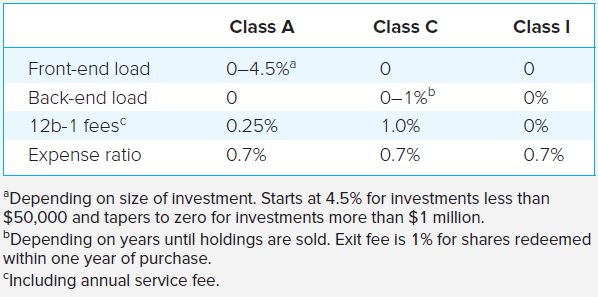
\includegraphics[keepaspectratio]{img//market_MF_Fees.png}}

\begin{center}\rule{0.5\linewidth}{0.5pt}\end{center}

\subsection{Impact of Costs on Investment
Performance}\label{impact-of-costs-on-investment-performance}

\pandocbounded{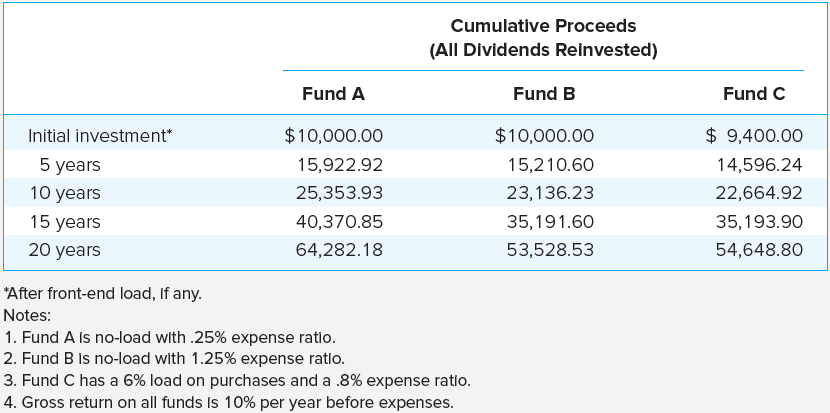
\includegraphics[keepaspectratio]{img//market_MF_Fees_Performance.png}}

\begin{itemize}
\tightlist
\item
  \textbf{Higher costs reduce net returns}.
\item
  \textbf{Lower-fee funds} outperform over time due to compounding
  effects.
\end{itemize}

\begin{center}\rule{0.5\linewidth}{0.5pt}\end{center}

\subsection{Comparing Share Classes: Equity Fund
Example*}\label{comparing-share-classes-equity-fund-example}

\textbf{Fee Structures}

\begin{itemize}
\tightlist
\item
  \textbf{Class A}: \textbf{4\% front-end load}, no ongoing fees.
\item
  \textbf{Class B}: \textbf{No front-end load}, but \textbf{0.5\% 12b-1
  fees} and a \textbf{declining back-end load}:

  \begin{itemize}
  \tightlist
  \item
    Starts at \textbf{5\%}, decreases \textbf{1\% per year} (until year
    5).
  \end{itemize}
\item
  \textbf{Fund Portfolio Return}: \textbf{10\% net of operating
  expenses}.
\end{itemize}

\textbf{Scenario: What Happens to a \$10,000 Investment?}

\begin{enumerate}
\def\labelenumi{\arabic{enumi}.}
\tightlist
\item
  \textbf{{[}1 year{]}}
\item
  \textbf{{[}4 years{]}}
\item
  \textbf{{[}10 years{]}}
\end{enumerate}

\textbf{Which share class provides higher net proceeds at different
investment horizons?}

\begin{center}\rule{0.5\linewidth}{0.5pt}\end{center}

\subsection{Investment Companies: Market
Size}\label{investment-companies-market-size}

\pandocbounded{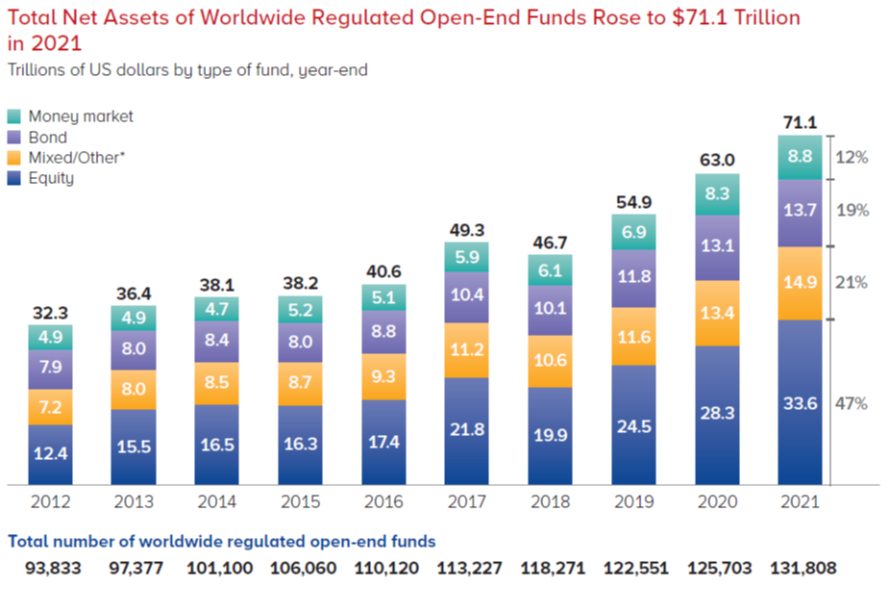
\includegraphics[keepaspectratio]{img//market_MF_Size.png}}

\begin{center}\rule{0.5\linewidth}{0.5pt}\end{center}

\subsubsection{Investment Companies: By
Region}\label{investment-companies-by-region}

\pandocbounded{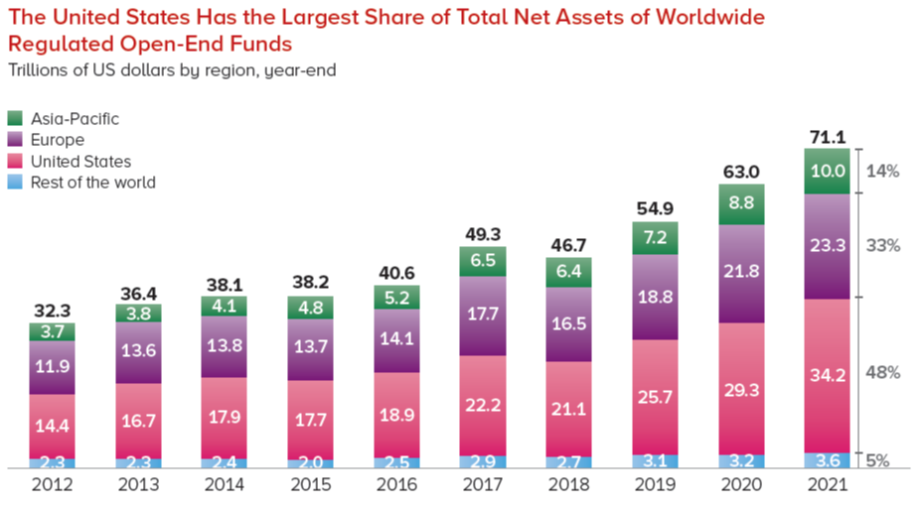
\includegraphics[keepaspectratio]{img//market_MF_By_Region.png}}

\begin{center}\rule{0.5\linewidth}{0.5pt}\end{center}

\subsection{Investment Companies: Recent
Development}\label{investment-companies-recent-development}

\begin{itemize}
\item
  \textbf{Exchange-Traded Funds (ETFs)}:

  \begin{itemize}
  \item
    Trade continuously like stocks.
  \item
    Can be sold short or purchased on margin.
  \item
    Generally lower costs than mutual funds.
  \item
    \textbf{Advantages of ETFs}:

    \begin{itemize}
    \tightlist
    \item
      More flexible than index funds.
    \item
      Lower expense ratios than actively managed mutual funds.
    \item
      Tax efficiency due to in-kind redemptions.
    \end{itemize}
  \item
    \textbf{Disadvantages of ETFs}:

    \begin{itemize}
    \tightlist
    \item
      Prices may deviate from \textbf{Net Asset Value (NAV)}.
    \item
      Must be purchased through a broker, incurring trading costs.
    \end{itemize}
  \end{itemize}
\item
  \textbf{Actively Managed ETFs}

  \begin{itemize}
  \item
    Traditionally, ETFs were required to track \textbf{specified
    indexes}.
  \item
    Recent expansion includes \textbf{actively managed ETFs} that follow
    different investment strategies:

    \begin{itemize}
    \tightlist
    \item
      Value investing
    \item
      Growth stocks
    \item
      Dividend yield
    \item
      Liquidity factors
    \item
      Recent performance trends
    \item
      Volatility
    \end{itemize}
  \item
    \textbf{Key Feature}:

    \begin{itemize}
    \tightlist
    \item
      Unlike traditional mutual funds, actively managed ETFs
      \textbf{disclose their portfolio composition daily}.
    \end{itemize}
  \end{itemize}
\item
  \textbf{Non-Transparent Actively Managed ETFs}

  \begin{itemize}
  \tightlist
  \item
    \textbf{Challenge}: Frequent portfolio disclosure could allow
    competitors to exploit fund trading strategies.
  \item
    \textbf{Solution}: Development of \textbf{non-transparent actively
    managed ETFs}.
  \item
    \textbf{Regulatory Approval}:

    \begin{itemize}
    \tightlist
    \item
      In 2014, the SEC granted permission to Eaton Vance to introduce an
      actively managed \textbf{non-transparent ETF}.
    \item
      \textbf{NextShares} began trading in 2016.
    \end{itemize}
  \item
    \textbf{Key Difference}:

    \begin{itemize}
    \tightlist
    \item
      Unlike traditional ETFs, these funds limit portfolio disclosure to
      protect trading strategies.
    \end{itemize}
  \end{itemize}
\end{itemize}

\begin{center}\rule{0.5\linewidth}{0.5pt}\end{center}

\subsection{Investment Companies: ETF
Trends}\label{investment-companies-etf-trends}

\pandocbounded{\includegraphics[keepaspectratio]{img//market_ETF_Size.png}}

Source: Statistica - Global exchange-traded funds (ETFs) from 2003 to
2021

\begin{center}\rule{0.5\linewidth}{0.5pt}\end{center}

\subsection{Investment Companies: Mutual Fund
Performance}\label{investment-companies-mutual-fund-performance}

\pandocbounded{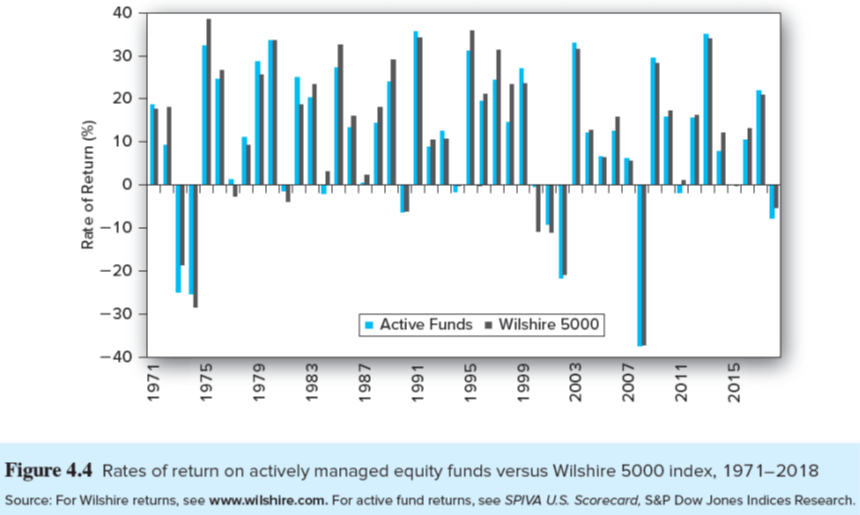
\includegraphics[keepaspectratio]{img//market_MF_Performance.png}}

\begin{center}\rule{0.5\linewidth}{0.5pt}\end{center}

\subsection{Investment Companies: Performance
Persistence}\label{investment-companies-performance-persistence}

\pandocbounded{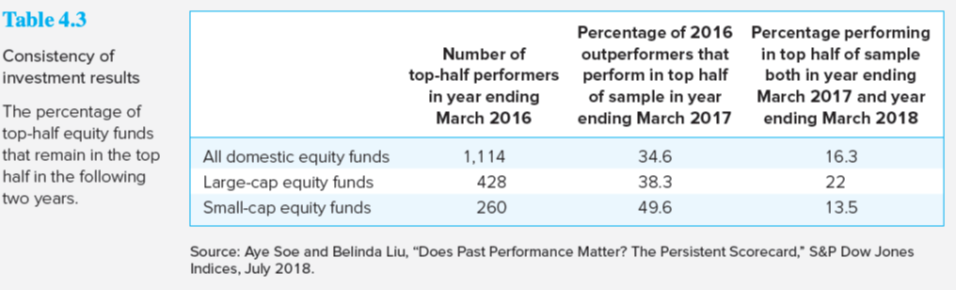
\includegraphics[keepaspectratio]{img//market_MF_Persistence.png}}

\begin{center}\rule{0.5\linewidth}{0.5pt}\end{center}

\subsection{Investment Companies: Closed-end
Funds}\label{investment-companies-closed-end-funds}

\pandocbounded{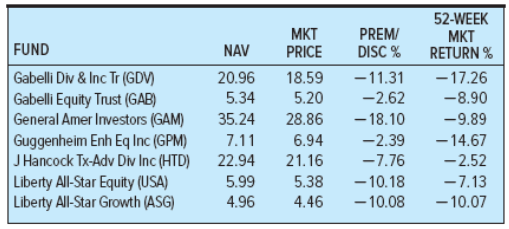
\includegraphics[keepaspectratio]{img//market_Closed_End.png}}

\begin{itemize}
\item
  Closed-end Fund Puzzle

  \begin{itemize}
  \tightlist
  \item
    The common divergence of price from net asset value, often by wide
    margins, is a puzzle that has yet to be fully explained
  \end{itemize}
\end{itemize}

\begin{center}\rule{0.5\linewidth}{0.5pt}\end{center}

\subsection{Investment Companies: Hedge
Funds}\label{investment-companies-hedge-funds}

\begin{itemize}
\tightlist
\item
  \textbf{Hedge Funds}:

  \begin{itemize}
  \tightlist
  \item
    Typically structured as \textbf{private partnerships}.
  \item
    Subject to \textbf{minimal regulation}, unlike mutual funds.
  \item
    Can pursue \textbf{complex investment strategies}:

    \begin{itemize}
    \tightlist
    \item
      Heavy use of \textbf{derivatives}.
    \item
      \textbf{Short selling}.
    \item
      \textbf{Leverage} to amplify returns.
    \end{itemize}
  \item
    Not available to the general public; open only to \textbf{wealthy or
    institutional investors}.
  \end{itemize}
\item
  \textbf{Lock-Up Periods}:

  \begin{itemize}
  \tightlist
  \item
    Many hedge funds require an initial \textbf{``lock-up'' period} of
    several years.
  \item
    Investors cannot withdraw funds during this time.
  \item
    Allows hedge funds to invest in \textbf{illiquid assets} without
    facing immediate redemption pressure.
  \end{itemize}
\end{itemize}

\begin{center}\rule{0.5\linewidth}{0.5pt}\end{center}

\subsection{References}\label{references}

\begin{itemize}
\tightlist
\item
  \href{https://www.bok.or.kr/portal/bbs/P0000603/list.do?menuNo=200460}{Financial
  Markets in Korea (Bank of Korea)}
\item
  \href{https://ktb.moef.go.kr/eng/main.do}{Korea Treasury Bonds
  (Ministry of Economy and Finance)}
\item
  \href{https://www.sifma.org/resources/research/fact-book/}{Capital
  Market Factbook (SIFMA)}
\item
  \href{http://global.krx.co.kr/}{The Korea Exchange (KRX)}
\item
  \href{https://www.icifactbook.org/}{Investment Company Factbook (ICI)}
\end{itemize}




\end{document}
